\documentclass[a4paper,14pt]{extarticle}
\usepackage{fontspec}
\usepackage{graphicx}
% настраиваем поля
\usepackage[left=30mm, right=10mm, top=20mm, bottom=20mm]{geometry}

% математический пакет
\usepackage{amsmath}
\usepackage{ dsfont }

% для того чтобы в adobe acrobat файл открывался в масштабе 100 процентов
\usepackage{hyperref}
\hypersetup{pdfstartview={XYZ null null 1.00}}

% устанавливаем Times New Roman и математический шрифт сочетающийся с ним
\setmainfont{Times New Roman}
\usepackage{newtxmath}

% локализация некоторых названий
\renewcommand\contentsname{Содержание}
\renewcommand\refname{Список используемой литературы}

% избавляемся от переполнение
\sloppy

%\полуторный интервал
\linespread{1.3} 

\begin{document}

% титульник
\thispagestyle{empty}

\begin{center}
    ФЕДЕРАЛЬНОЕ ГОСУДАРСТВЕННОЕ АВТОНОМНОЕ\\
    ОБРАЗОВАТЕЛЬНОЕ УЧРЕЖДЕНИЕ\\
    ВЫСШЕГО ОБРАЗОВАНИЯ\\
    «НАЦИОНАЛЬНЫЙ ИССЛЕДОВАТЕЛЬСКИЙ УНИВЕРСИТЕТ\\
    «ВЫСШАЯ ШКОЛА ЭКОНОМИКИ»
\end{center}

\vfill

\begin{center}
    \textbf{Факультет информатики, математики и компьютерных наук}

    \vspace{20pt}

    \textbf{Программа подготовки бакалавров по направлению \\
    01.03.02 Прикладная математика и информатика}
\end{center}

\vfill

\begin{center}
    \textit{Харчиков Игорь Владиславович} 
    
    \vspace{20pt}
    
    \textbf{КУРСОВАЯ РАБОТА}

    \vspace{20pt}
    
    Медицинская классификация на основе описания состояния пациента с использованием модели на базе BERT
\end{center}

\vfill

\begin{flushright}
Научный руководитель

\vspace{5pt}

к.т.н., старший преподаватель 
\\
кафедры ПМИ
\\
Cеменов Дмитрий Павлович
\end{flushright}

\vfill

\begin{center}
    Нижний Новгород, 2023
\end{center}
\newpage

% содержание
\tableofcontents
\newpage

% введение
\section*{Введение}
% добавляем введение в содержание
\addcontentsline{toc}{section}{Введение}
Методы машинного обучения значительно помогаеют в автоматизации многиъ процессов, с некоторого времени, алгоритмы машинного и глубинного обучения стали обладать достаточными возможностями и надежностью для применения и в сфере медицины \cite{med_survey}. \newline
Медицина является достаточно обширной сферой как науки так и поведневной деятельности, ее аналитическая часть часто взаимодействует с большим количесвтом наблюдений разного рода, как в масштабах популяций, так и одного пациента. Даже один единственный пациент может пройти такое количество анализов, что понадобится достаточно продолжительное время и целый набор специалистов для постановки диагноза. Медицинские обследования пораждают данные в разных формах, включая, но не ограничиваяь табличными данными на разного рода тестах, визуальной информацией в в виде снимков, временных рядов при анализе разного рода биоритмов. 
Но еще до такого рода информации, о пациенте получают более сложно поддающуюся анализу, но легкодоступную ифнормацию - из разговор при визите ко врачу.\newline
Из рассказа пациента о своем состоянии, можно сделать выводы о возможных заболеваниях, вычленить ключевые и формализованные симптомы, которые понадобятся для ведения истории и дальнейшего направления на анализы и ведения пациента в целом. Бывшая актуальной во все времена проблема распознавания такого рода обостряется с развитием телемедицины - то есть обращении при отсутствии очного посещения врача. Доступность пораждает больший спрос и задача формализации каждого случая становится еще острее. Более того, процесс может быть автоматизирован рекоммендательной интеллектуальной системой для дальнейшего направления, или предложения направиться на анализы, тогда и для нее понадобится формальный список аномалий в состоянии пациента.
\newline
Только недавние достижения искуственного интеллекта позволили эффективно и надежно работать с такими данными. Работа с текстами на "человеческом языке" называется "обработкой естественного языка" (далее - Natural Language Processing или сокращенно NLP). значительный прорыв в области обработки такого рода данных связан с развитием глубинного обучения и дальнейшим появлением рекуррентных сетей и архитектур на основе механизма внимания.
\newline
Также важно отметить проблему сокрытости зананий нейронной сети. Эти алгоритмы представляют Black Box функции, то есть неизвестен смысл их внутренних процессов. Это неприемлимо при применении в задачах реальной жизни, тем более в медецинской сфере. Поэтому требуется дополнительное исследование и интерпретация обученной модели. В случае имплементации в рабочий процесс, эксперты должны иметь возможность оценивать, как алгоритм работает с данными для валидации верности работы, для этого не достаточно обычных метрик.
\newline
Цели работы:
\begin{enumerate}
\item  Формализация NLP-задачи для ML и обзор технологий для решения
\item  Механизмы стоящие за RNN и Transformer, изучение основных механизмов и архитектур для актуальных нейронных сетей в сфере NLP
\item  Осуществить файн-тюнинг на основе претренированной языковой модели BERT для решения задачи классификации на медицинских данных в виде естественного языка
\item  Применяя инструменты анализа алгоритмов глубинного обучения интерпретировать связи, созданные внутри нейронной сети
\end{enumerate}

% добавляем главы
\section{Естественный язык как модальность данных и примененимость методов машинного обучения}
\subsection{Специфика репрезентации данных}
Как уже было сказано, обработка естественного языка NLP одна из самых актуальных в настоящее время. Выше было отмечено, что NLP это сложный процесс, ключевыми сложностями вызванными непосредственно природой данных, являются кодирование данных и работа с непостоянной размерностью. Фраза на естественном языке - это последовательность слов некоторого языка, но для любого алоритма потребуется каким-то образом перевести ее в числовой тип, единственный принимаеиый существующими алгоритмами. Слова крайне враждебны в этом отношении, наивные методы крайне неэффективны, и, чтобы покрыть целый словарь, понадобится очень много памяти, более того, фраза даже из закодированных слов имеет нефиксированную длину. 
В итоге при подготовке данных для решения встает два вопроса:
\begin{itemize}
    \item Какой метод кодирования слов оптимален в терминах сохранения информации и эффективности хранения
    \item Как обработать последовательность нефиксированной длины или преобразовать ее таким образом, чтобы размерность данных стала фиксированной
\end{itemize}
Последний вопрос еще более важен, так как он непосредственно связан с моделью для решения задачи.
\subsection{Механизмы кодирования и репрезентации в качестве многомерных объектов}
Для какой-либо задачи в области NLP будет определен некоторый конечный словарь - множество всех допустимых встречающихся слов естественного языка. Очевидным методом является применение кодирования OneHotEncoding (далее OHE), при котором $i$-ому слову будет соответсвовать вектор состоящий из нулей с $i$-ым элементом единицей, то есть: 
\begin{equation} \label{ohe_eq} 
\text{\textit{Для словаря}}\ V, |V| = N \ \exists \ ohe:V \longrightarrow \mathds{R}^{N}; ohe(V_{i}) = a, \forall j \neq i a_{j}=0,\ a_{i} = 1 
\end{equation}

Отображение \ref{ohe_eq} позволяет получить численное представление слов в виде векторов, однако размерность равна таковой у словаря.

От части эту проблему можно решить при помощи грамотного разделения фраз на слова. Вместо наивного разбиения на непосредственные слова (разделенные в языке пробелами) и знаки пунктуации можно сократить длину словаря при помощи \textit{токенизации}. Алгоритмы токенизации могут быть разными, помимо сокращения мощности множества слов токенизация может так же сообщать полезную информацию алгоритмы, как будет показанно позже. \newline
Как самостятельный контейнер информации one-hot вектор не несет смысла, кроме явного указания на то, что за слово было закодировано. Полезным преобразованием является векторизация слова (Word To Vector - далее W2V)\cite{w2v}. W2V является обучаемой системой, которая отображает токены в вектора фиксированной размерности, являющейся гиперпараметром. В итоге обучения получается матрица весов $W_{N \times S}$, алгоритм устроен таким образом, что при помощи прохода окном по послеовательности токенов, максимизируются условные вероятности появления слова из центра окна в окржении остальных слов из окна. Таким образом, выявляется контекстная значимость слов. Векторы полученные данным алгоритмом обладают удобными свойствами, в частности компактность относительно семантического значения, то есть блзкие по смысловому значению слова отобразятся в близкие векторы. 
\begin{equation} \label{w2v} 
\text{\textit{Для словаря}}\ V, |V| = N \ w2v_{S}:V \longrightarrow \mathds{R}^{S},\ S \in \mathds{N};
w2v_{S}(V_{i}) = ohe(v_{i})\times W_{N \times S} = b \in \mathds{R}^{S}
\end{equation}
Усовершенствованием технологии является FastText \cite{ft} помимо улучшенного процесса обучения применяющий дополнительно подобие токенизации, разбивая слова на части. Это позволяет более эффективно обрабатывать неизвестные слова, так как они могут состоять из встреченных ранее токенов, и выделяет больше информации за счет работы с уровнем, ниже слов естесвенного языка.
Таким образом, для работы классических методов машинного обучения можно получить векторное представление фразы в виде последовательности векторов, а затем каким либо образом преобразовать в единственный вектор при помощи поэлементного среднего:
\begin{align*} 
x = \frac{ \sum_{i=1}^{M} v2w_{S}(v_{i}) }{M} \in \mathds{R}^{S}
\end{align*}
Для методов глубинного обучения инструментарий кодирования может использоваться такой же, однако для наиболее эффективных и рассмотренных далее в работе архитектур он немного отличается. Важно отметить, что методы глубинного обучения обыкновенно оперируют всей последовательностью, не сводя ее к одному вектору. Как было отмечено в \cite{RNN_survey}, возможность оперировать всей последовательностью позволяет захватывать конекст последовательности, несмотря на очевидные плюсы алгоритмов, инвариантных к длине данных, они проигрывают в сфере восприятия и выделения черт (feature extraction).

Применяются достаточно продвинутые алгоритмы токенизации. BPE-токенизация \cite{bpe} применяется во многих популярных и мощных решениях, алгоритм очень эффективен засчет отыскания и жадного перекодирования наиболее частых пар токенов в новый токен, не встречавшийся ранее. Как и BPE Word Piece токенизация, впервые представленныя в \cite{word_piece}, разбивает последовательность на уровне ниже целых слов. Метод является усовершенствованной версией и вместо частоты в BPE оперирует вероятностным подходом. При выборе пар высчитывается правдоподобие - вероятность последовательного нахождения токенов друг за другом. Word Piece добавляет токены в словарь склеивая входные до тех пор, пока уровень правдоподобия не опустится до заранее выбранного порогого значения. Алгоритм так же является жадным, но в отличие от BPE итерации заданы не напрямую, а через выше обозначенный порог. 

Для векторизации токенов в нейронных сетях используют так же слой вложения (Embedding). Итоговое вычисление вложенного представления схоже с \ref{w2v}. Блок препроцессинга включен в саму сеть и обучается вместе с ним, от обычного линейного он также отличается оптимизацией для работы с разреженными данными.
При кодировании последовательности может оказаться так, что одинаковые векторы стоят на разных местах, то есть один и тот же токен может выполнять разную роль в одной фразе. Чтобы добавить информацию об относительном положении слова в последовательности, к каждому вектору добавляется значение полученное из позиционного кодирования (Positional Encoding или PE) поэлементным сложением. Значения вычисляются следующим образом \cite{transformer}\cite{pe}:\\
\textit{Пусть t - позиция в последовательности, d - размерность векторного представления, (i) - индекс элемента вектора} 
\begin{align*}
p_{t}^{(i)} = f(t)^{(i)} := 
\begin{cases} 
sin(w_{k} * t), & \textit{при } i=2k 
\\
cos(w_{k} * t), & \textit{при } i=2k +1
\end{cases}
\textit{, где }
w_{k} = \frac{1}{1000^{2k/d}}
\end{align*}
\newline
Пример полученных значений - \ref{pe_vals}.
\begin{figure}[h]
\caption{Спектр значений позиционного кодирования с размерностью (Depth) 128 и максимальной длинной (Position) 50, каждая строка - вектор $p_{t}$}
\centering
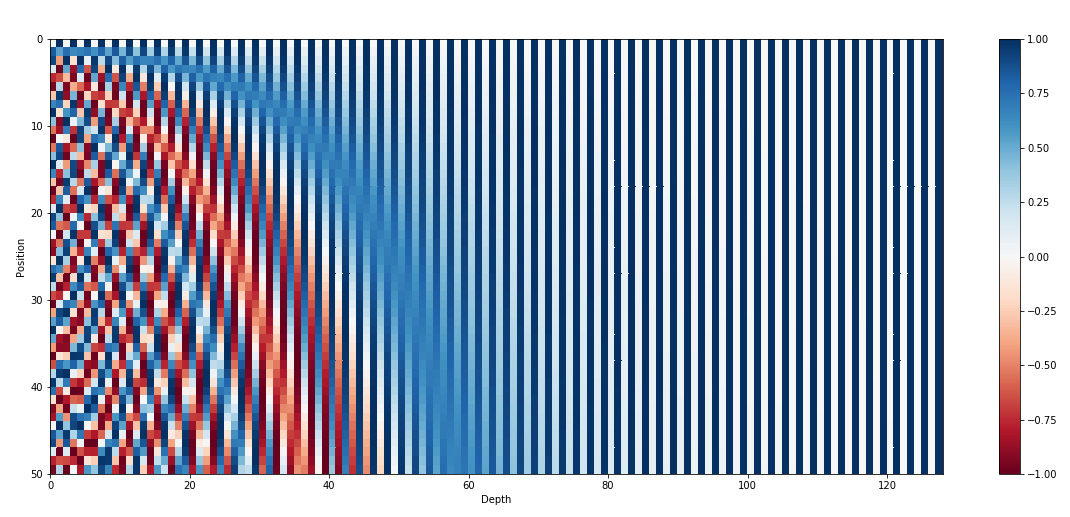
\includegraphics[width=1\textwidth]{positional_encoding.png}
\label{pe_vals}
\end{figure}
\newline
\section{Рекуррентные сети и  трансформерные архитектуры}
\subsection{Развитие идей и инструментов обработки последовательностей}
\subsubsection{Энкодер-Декодер архитектура}
Как было подчеркнуто в предыдущей главе, ссылаясь на \cite{RNN_survey}, алгоритмы не инвариантные к длине последовательности выигрывают по многим возможностям. Скрытые Марковские Модели, или кратко СММ, относятся к такому типу алгоритмов. Однако в них состояние модели зависит только от предыдущего, хотя и существуют модификации расширяющие возможности. Рекуррентные архитектуры нейронных сетей с механизмом LSTM (Long Short Term Memory unit - Механизм Короткой Долгосрочной Памяти) предложенным в \cite{LSTM} обладают возможностью сохранять контекст на протяжении обработки всей последовательности. LSTM не является единственной опцией, и даже он имеет множество модификаций, однако так или иначе все рекуррентные сети отдельно обрабатывают каждый токен, но каким-либо образом учитывают информацию о предыдущих. После прохождения по последовательности вложенное представление последнего токена будет обладать информацией о всей последовательности. Более того, такое представление будет обладать все тем же свойством "семантической компактности" как и отображение \ref{w2v}, однако уже в масштабе целого предложения.
Помимо того, что это само по себе очень полезное свойство, на нем основано главное преумещство энкодер-декодерных архитектур на основе рекуррентных операторов.
\newline
\begin{figure}[h]
\caption{Архитектура RNN для seq2seq задачи, развернутая по ходу последовательности}
\centering
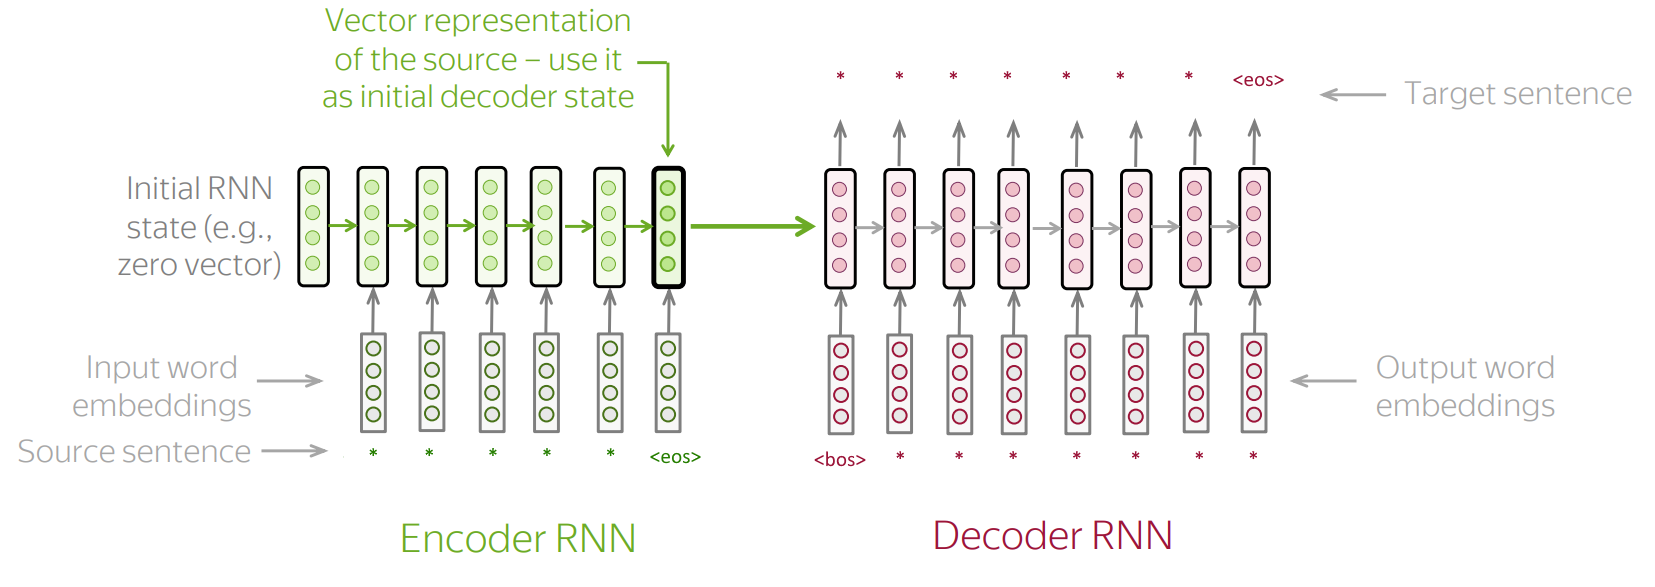
\includegraphics[width=0.75\textwidth]{rnn_arch_base.png}
\label{rnn_arch}
\end{figure}
\newline
Наиболее яркое применение этой архитектуры связано с задачей seq2seq (sequence to sequence или перевод последовательности в последовательность). Последнее соятояние энкодера используется как инициализация для состояний декодера, передавая таким образом информацию для создания новой последовательности извлеченную из входной. Эффективно, это создает "бутылочное горлышко" для сети, заставляя ее наиболее эффективно отражать в этом векторе информацию из последовательности на входе.
\newline
Если задача требует не создан ие новой последовательности, но декодер заменяется на другие операторы, которые будет взаимодействовать как раз таки с последним состоянием последнего слоя энкодера, или его аналогом, как будет показано далее, как с самым информативным и полным представлением об оригинальной последовательности.
\newline
При этом итерация по последовательности может быть как в одну сторону - от начала к концу или наоборот, так и вместе, после чего вложенные преддставления будут сконкатенированны. Такой алгоритм будет называться \textit{Двунаправленным (Bidirectional)}.
% \subsubsection{LSTM}
% \cite{RNN_survey}
\subsubsection{Применение механизма внимания}
Прорывным шагом в работе с энкодер-декодерной архитектурой являлся миханизм внимания\cite{Attention}. Он позволяет не просто использовать последнее состояние энкодера, но управлять тем, какие состояния предыдущего слоя и как использовать, за счет вычисления значимости внимания (Attention Scores) вычислимых между всеми элементами текущей и прошлой последовательностей.
\newline
Гладким аналагом максимума является функция \textit{Softmax}, она и используется для получения значимости внимания:
\begin{equation} \label{softmax} 
\nonumber A \in \mathds{R}^{S}: Softmax(A_{i}) = \frac{A_{i}}_{\sum_{j=1}^{S}exp(A_{j})}
\end{equation}
\textit{Q - Query}, член для которого ведутся вычисления на данном шаге, \textit{K - Key} - все члены последовательности, по которым итеративно идет вычесление, используются для получения значимости внимания между членами; \textit{V - Value} - значение, используемое далее в вычислениях.
Итоговая формула:
\begin{gather} \label{dot_product_att_w/o_scale} 
Attention(Q,K,V) = Softmax \left(QK^{T}\right)V\\
\nonumber \textit{Здесь и далее } d_{k}, d_{v} \in \mathds{N}; Q, K \in \mathds{R}^{d_{k}}, V \in \mathds{R}^{d_{v}}
\end{gather}
Применение механизма внимания отражено на \ref{attn_usg}.

\begin{figure}[h]
\caption{Применение механизма внимания в двунаправленной RNN с MLP - линейными слоями, разделенными активацией-гиперболическим тангенсом,\cite{Attention}}
\centering
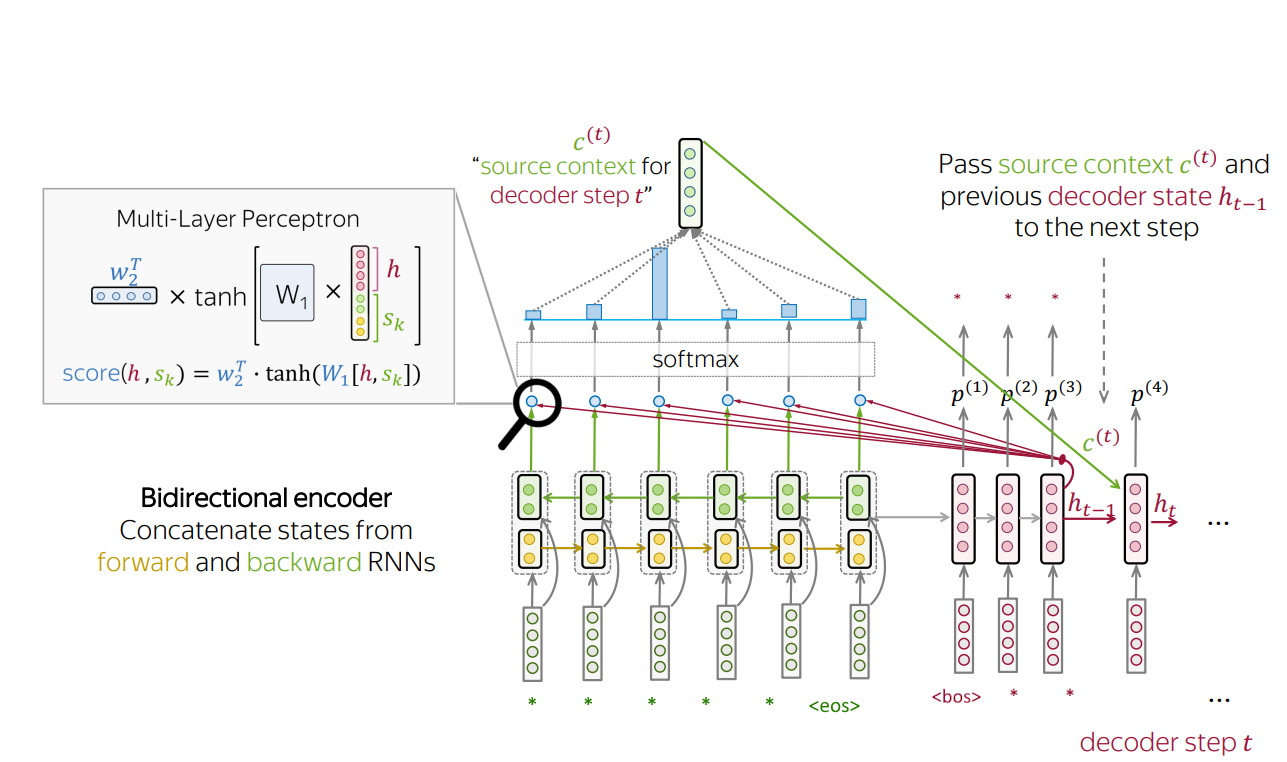
\includegraphics[width=1\textwidth]{attn_usg.png}
\label{attn_usg}
\end{figure}

\subsubsection{Трансформерная архитектура}
В архитектуре трансформерной сети \cite{transformer} нет обычных операторов рекуррентной сети, но используется механизм внимания с множителем для нормализации значений:
\begin{equation} \label{dot_product_att_w/_scale} 
Attention(Q,K,V) = Softmax \left(\frac{QK^{T}}_{\sqrt{d_{k}}}\right)V
\end{equation}
При этом внимание внутри энкодера и декодера применяется с \textit{Q=K=V} и называется \textit{Self-Attention}. Между энкодером и декодером есть связующий мезанизм внимания, где \textit{Q} используется из декодера а \textit{K,V} из энкодера \ref{transformer}.\newline
Так же для больших выразительных способностей внимания, используется версия с множеством голов \textit{h}:
\begin{gather} \label{mh_att} 
\nonumber \textit{}\\
MultiHeadAttention(Q,K,V) = \bigoplus^{h}_{i=0}\left(head_{i}\right)W_{0},\\
\nonumber head_{i} = Attention\left( QW_{i}^{Q},KW_{i}^{K},VW_{i}^{V}\right) - \textit{аналогично \ref{dot_product_att_w/_scale} от линейных }\\ 
\nonumber \textit{комбинаций с собственными весами}
\end{gather}
Наличие разных голов помогает выделять разные типы взаимосвязей между членами последовательности.
\begin{figure}[h]
\caption{Архитектура трансформера}
\centering
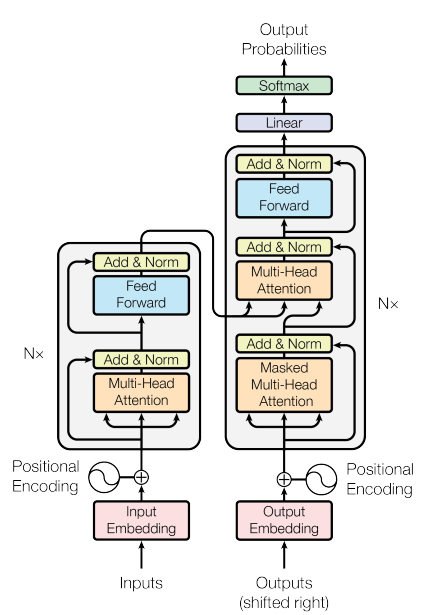
\includegraphics[width=0.37\textwidth]{transformer.png}
\label{transformer}
\end{figure}
\subsection{Технология обучения BERT}
Наиболее мощная претренерованная модель трансформера представлена в \cite{bert}. 
При токенизации добавляются специальные сегментационные токены \textit{[CLS]} и \textit{[SEP]}; первый ставится в начале последовательности, второй отделяет значимые части при работе сразу с двумя последовательностями для задачи с ответом на вопрос (где и разделяетответ и вопрос).
\begin{figure}[h]
\caption{Токенизация в BERT}
\centering
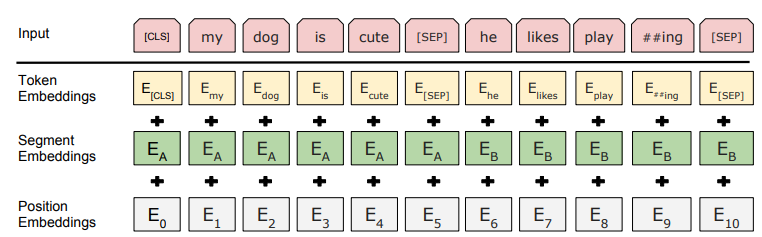
\includegraphics[width=0.75\textwidth]{bert_token.png}
\label{bert_token}
\end{figure}
Для обучения сети без учителя, из входных данных случайно удаляются некоторые члены, их заменяют специальным токеном \textit{[MASK]}. 
\begin{figure}[h]
\caption{Обучение без учителя с масками}
\centering
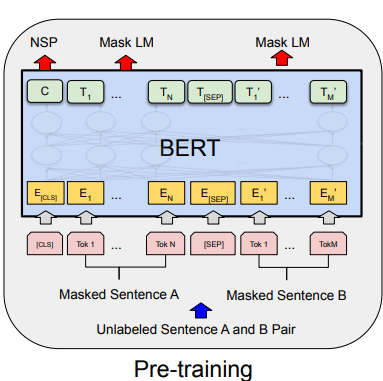
\includegraphics[width=0.5\textwidth]{MLM.png}
\label{mlm}
\end{figure}
Целью сети становится восстановление токенов, сокрытых \textit{[MASK]}, то есть макчимизацией вероятности выбрать правильное слова из словаря на эту позицию. Такой подход позволил обработать большое количество данных без разметки и получить очень сильную модель, которую в процессе тонкой настройки \textit{fine-tuning} можно подготовить для любой задачи в сфере NLP. Очень мощное представление о входных данных будет содержаться в выходном \textit{[CLS]} токене - специальном токене для классификации. Свойства представления данных в нем cхоже с "бутылочным горлышком" в энкодер-декодерных архитектурах.
\section{Применение BERT к медицинским данным}
\subsection{Формализация задачи и обзор данных}
\subsubsection{Датасет NBME}
NBME \cite{NBME} выбран в качестве датасета для проверки алгоритма и последующей интрепретации. Задача связана с формализацией диагноза из опроса и осмотра пациента. 
В качестве данных представлены заметки о пациентах - отрывки наблюдений о каждом и признаки для каждого клинического случая, эти данные разделены на две таблицы.
\newline
Понятия о данных этого датасета:
\begin{itemize}
\item Клинический случай (clinical case): сценарий (например, симптомы, жалобы, опасения), который пациент представляет.
\item Примечание пациента (patient notes): Текст, содержащий подробную важную информацию, сообщенную пациентом во время встречи (физического осмотра и собеседования).
\item Признак (feature): Клинически значимая концепция. В рубрике описаны ключевые понятия, относящиеся к каждому конкретному случаю.
\end{itemize}
Обучающая и тестовые выборки разбивают данные по клиническому случаю, примечанию пациента и признаку (либо признакам), задача заключается в указании части примечания, содержащей информацию о признаке. 
\subsubsection{Постановка и метрика качества}
Ответы представлены парами индексов \textit{\{ i, k \}}, возможно несколько для 1 сэмпла. Как раз такие пары и должна научиться строить модель.
Задача не очевидна, но ее можно свести к классификации посредствам перехода к следующему восприятию ответов:
позитивным сэмплом (речь о сабсэмпле-индексе для реального сэмпла) называть входящие в обозначеный выколотый справа отрезок индексы; по факту от модели требуется бинарно классифицировать все индексы, вместо пары \textit{\{ i, k \}} максимизируя вероятности для $\forall k \in [i,j)$ для верных.
\newline
Предложенная метрика для данных в соответствующем данным соревнованию - специально заданная \textit{f1score}. Обычный вид метрики:
\begin{gather*}
    \textit{TP - верно предсказанный позитивный сэмпл,}\\ 
    \textit{FP - неверно предсказанный позитивный сэмпл,}\\
    \textit{FN - неверно предсказанный негативный сэмпл}\\
    \nonumber Recall = \frac{TP}{TP+FN}\\
    \nonumber Precision = \frac{TP}{TP+FP}\\
    f1score = 2*\frac{Recall*Precision}{Recall+Precision}
\end{gather*}
Метрика для этой задачи имеет такую же формулу, но отличается более подходящим определением \textit{TP, FP, FN}:
\begin{gather*}
    \textit{TP - индекс входит в пересечение предсказания и лейбла,}\\
    \textit{FP - входит в предсказанный, но не в лейбл,}\\
    \textit{FN - входит в лейбл, но не в предсказанный срез}
\end{gather*}
Важное свойство метрики заключается в том, что она как среднегармоническое мягко приближает минимум метрик \textit{Полноты} и \textit{Точности}, достаточно справедливо оценивая качество модели в терминах ошибки первого и второго рода, что вытекает из стандартного определения и сохраняется в описанном для этой задачи. 
\newline
После выбора всех значащих индексов их нужно превести в вид \textit{\{ i, k \}} и разделить ";" для соответсвия требованиям при помощи несложного процесса парсинга.
% \subsubsection{Explanatory Data Analysis}
% Полезно может быть дополнительно исследовать данные, в ходе EDA можно получить какие-то важные характеристики.
\subsection{Решение задачи}
Для решения задачи использовался претренированая модель BERT Base Uncased и соответствующий токенайзер (работа проведена с использованием фреймворков \textit{pytorch} и \textit{hugging face transformers}). Поверх нее были добавлены 3 линейных слоя с дропаутом - оператором, случайно зануляющим некоторые каналы с вероятностью \textit{p} при тренеровке и домножающим остальные значения на $\frac{1}{1-p}$. Применение техники регуляризует сети по средствам контроля коадаптации искусственных нейронов.
\newline
Применяя \textit{[CLS]} токен и линейные слои получаются 1-мерные массивы, для получения вероятности требуется применить к ним фунцию $Sigmoid(x) = \frac{1}{1+e^{-x}}$. В качестве функции потерь применялась \textit{Бинарная Кросс Энтропия}:
\begin{equation} \label{BCE}
    BCE(x,y)=\{l_{j}\}, l_{j} = −w_{n}\left(y_{n}\times log x_{n}+(1−y_{n})\times log (1 - x_{n})\right)
\end{equation}
Для оптимизации весов в процессе обученния использовался \textit{AdamW}, версия оптимизатора с адаптивными моментами и переработанным механизмом регуляризации на основе весов сети, файн-тюнинг длился 3 эпохи с постоянным размером шага обучения $lr=10^{-5}$. Также для более стабильного процесса оптимизации приенялась техника \textit{клипинга градиента} - ограничения значений градиента пороговыми значениями ($grad := max(grad, threshhold)$), обеспечивающий более плавную сходимость без \textit{взрывов градиента}.
Результат на валидационной выборке после 3 эпох файнтюнинга:
\begin{center}
\begin{tabular}{ |c|c| } 
 \hline
 Метрика & Значение\\ 
 \hline
 Accuracy & 0.99307\\ 
 \hline
 Precision & 0.725280\\ 
 \hline
  Recall & 0.85514\\ 
 \hline
  f1 & 0.78488\\ 
 \hline
\end{tabular}
\end{center}

\begin{figure}[h]
\caption{Изменение функции потерь в ходе дообучения}
\centering
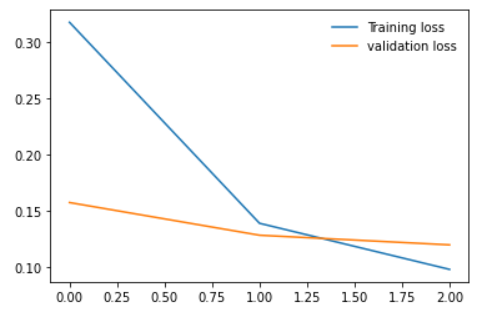
\includegraphics[width=0.5\textwidth]{loss_bert.png}
\label{loss}
\end{figure}
\newline
Текущий лучший результат на данных составляет \textbf{\textit{f1score} = 0.89592}. Несмотря на большой отрыв, полученная модель все равно обладает достаточным качеством, чтобы быть объектом интерпретации.
\subsection{Интерпретация алгоритма}
\subsubsection{Значение Шэпли}
Как было обозначенно в начале, алгоритмы требуется интерпретировать для последующей оценки реальными экспертами. Одним из основных методов является оценка влияния входных данных на результат. При помощи \textit{SHAP (SHapley Additive exPlanation)} можно оценить вклад входных признаков на ответ модели. Несмотря на то, что \textit{SHAP} предназначен для оценки вклада тгроков в каолиционной игре и вычисления основаны на расчете маржинального вклада игроков, при помощи интерпретации призников как игроков и вычисления маржинального вклада при помощи сэмплинга \cite{model_expl}, эти значения будут являться хорошим критерием при анализе модели машинного обучения\cite{shap_models}.
\subsubsection{Анализ модели при помощи SHAP}
Анализ BERT моделей с классификацией последовательности представленный в \cite{bert_shap} подразумевает вычисления для каждого токена входной последовательности. Для применения подхода к текущей задаче восприятие разметки как бинарной классификации каждого члена последовательности так же полезно. В данном случае вычислен \textit{SHAP} для пар элемент \textit{i} - вероятность для элемента \textit{j}.
\newline
В результате для предложения 
\begin{figure}[h]
\centering
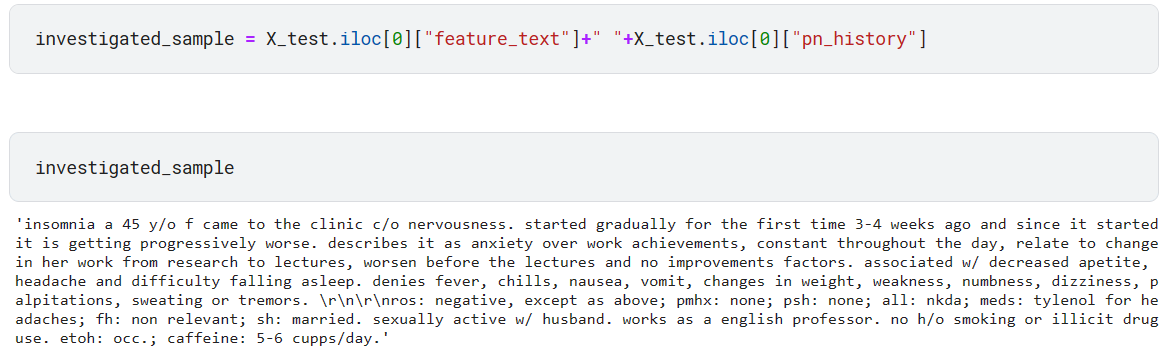
\includegraphics[width=0.75\textwidth]{sample.png}
\label{sample_txt}
\end{figure}
получилась матрица \ref{shap_mt}.

\begin{figure}[h]
\caption{Карта SHAP Values}
\centering
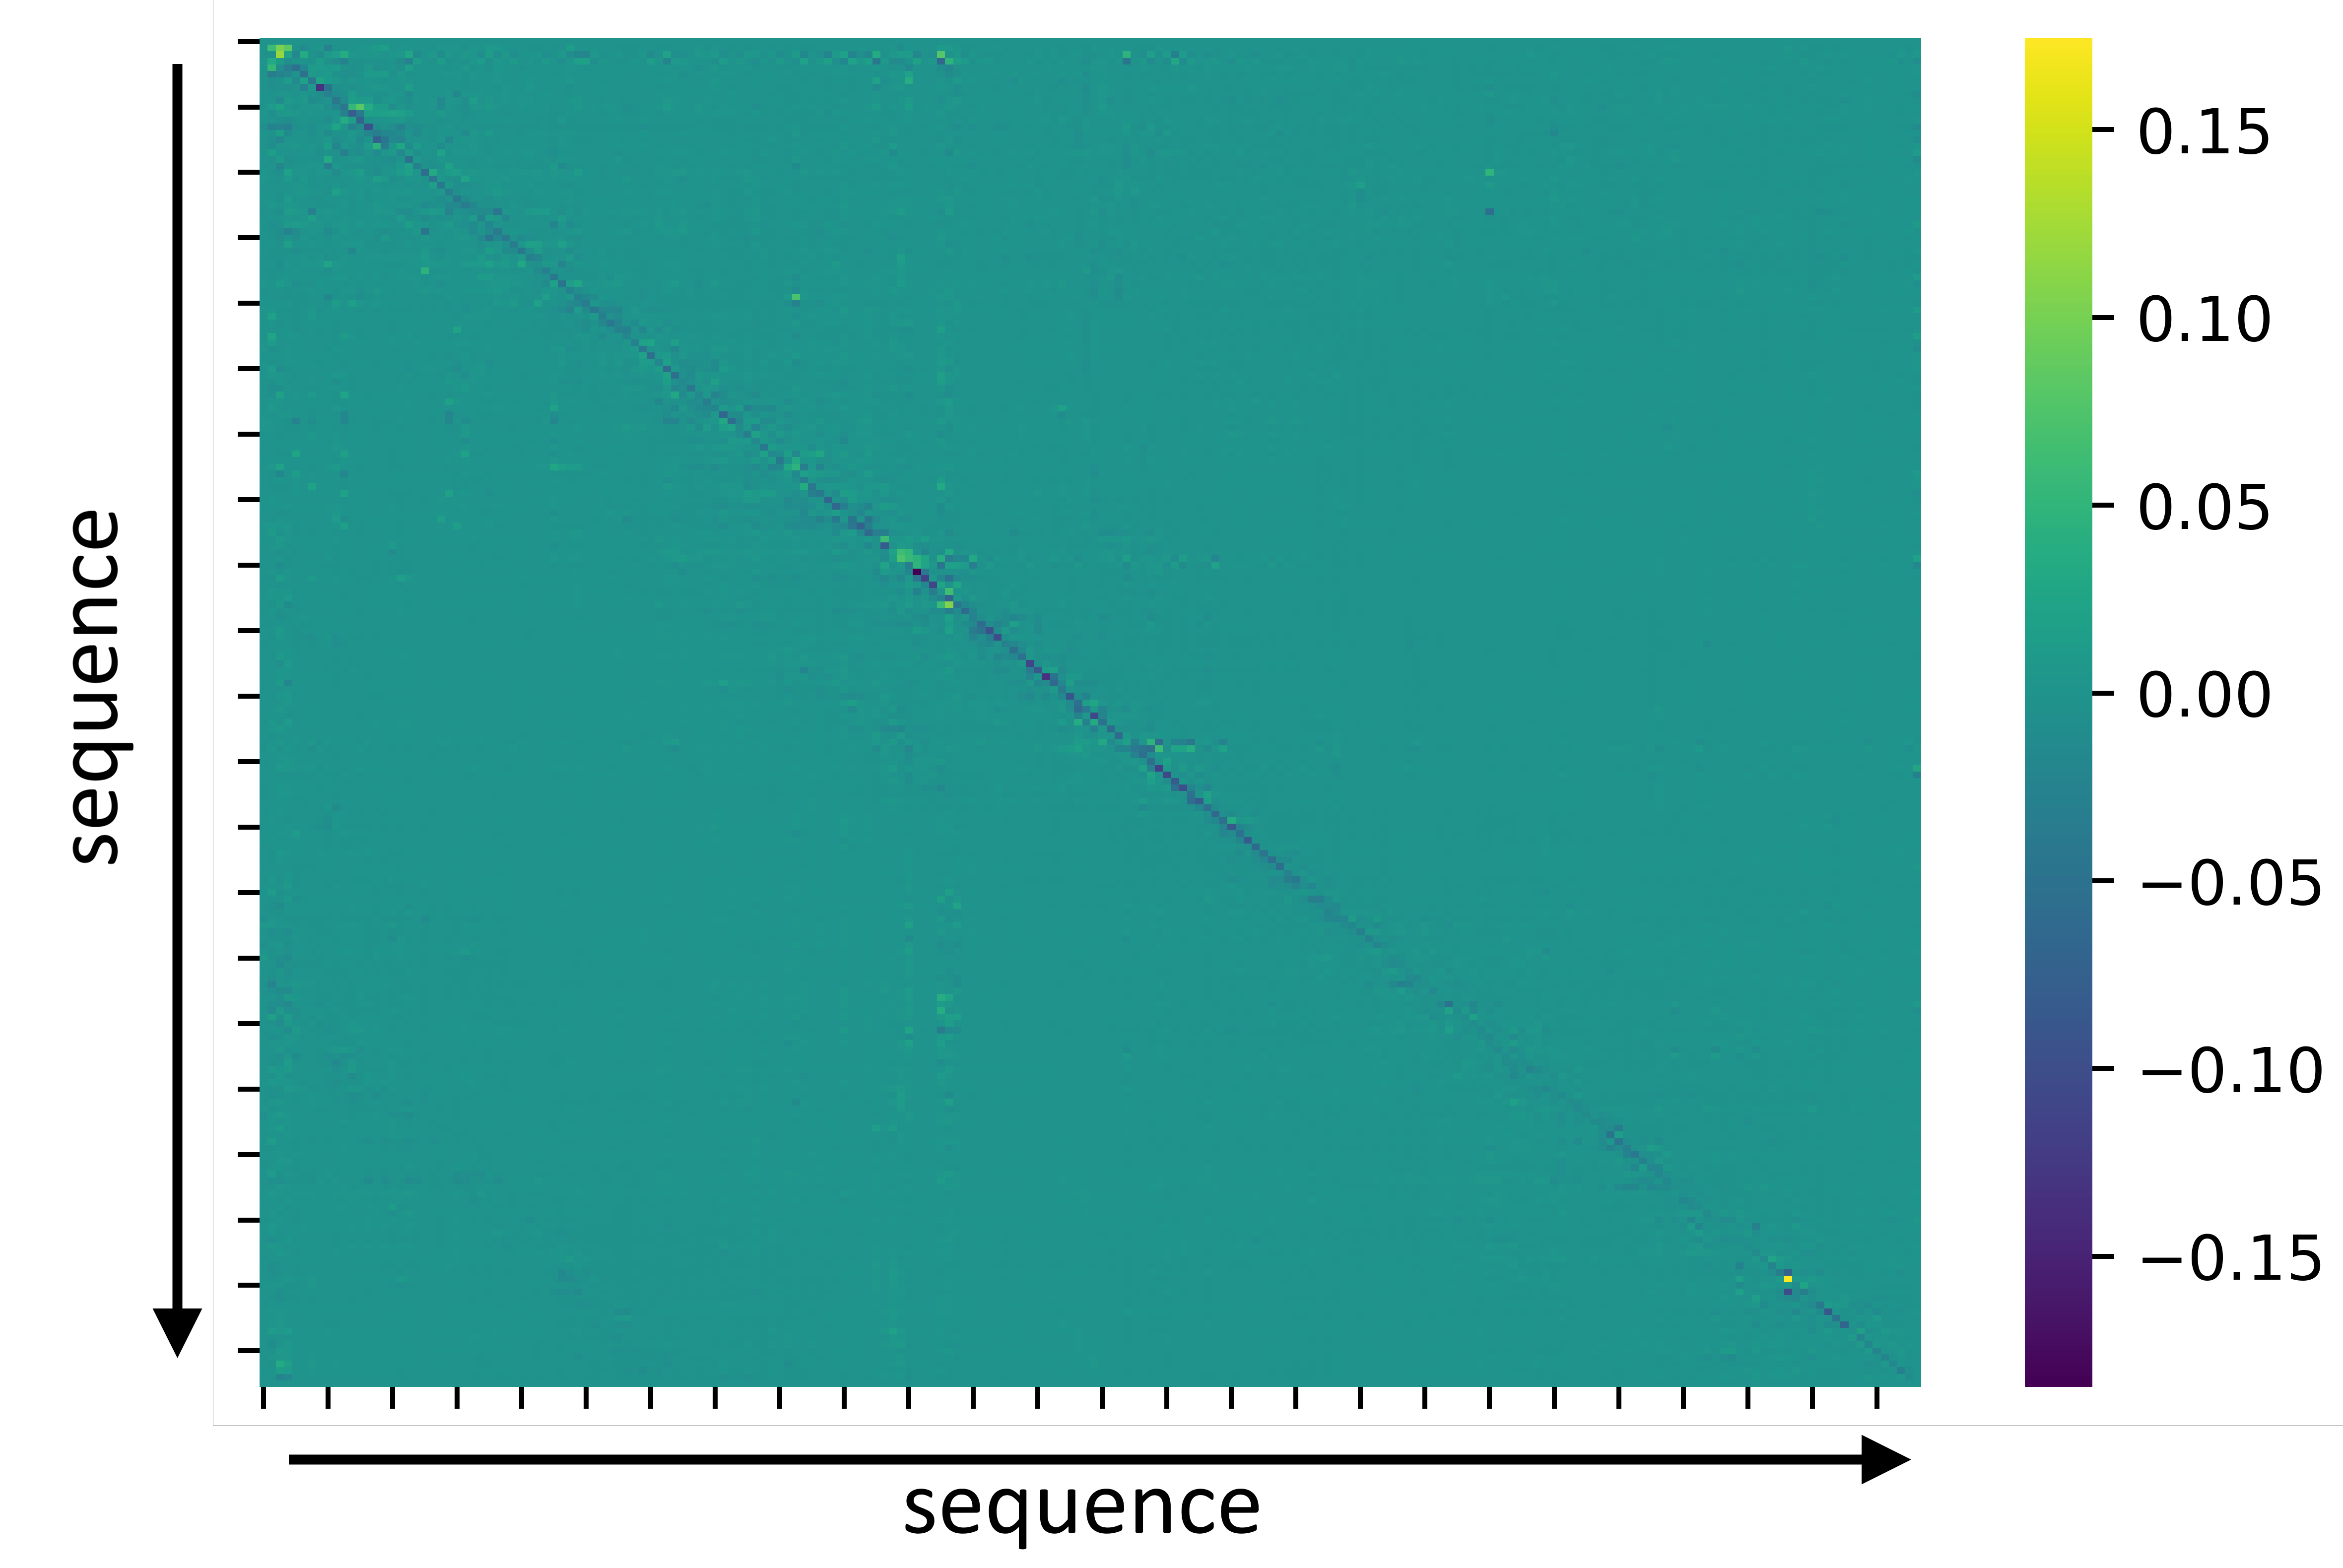
\includegraphics[width=1\textwidth]{sequence_shap_map.png}
\label{shap_mt}
\end{figure}
Пользуясь такой матрицей можно по индексу в последовательности найти слова, ответственные за принятие решения сетью и понять логику получения ответа для какого-то региона (возможная трактовка матрицы отражена на \ref{shap_mt_alloc}).
\begin{figure}[h]
\caption{Карта SHAP Values с выделениями: красными рамками выделены токены с повышенными положительными SHAP; \textit{a,b} и \textit{c} соответствуют 1 найденному региону, при этом элементы в \textit{b} наиболее близки к диагонали, то есть токены самого региона вложились в повышение вероятности, а \textit{a} и \textit{c} находятся ранее и после региона в последовательности, выступили в качестве контекста.}
\centering
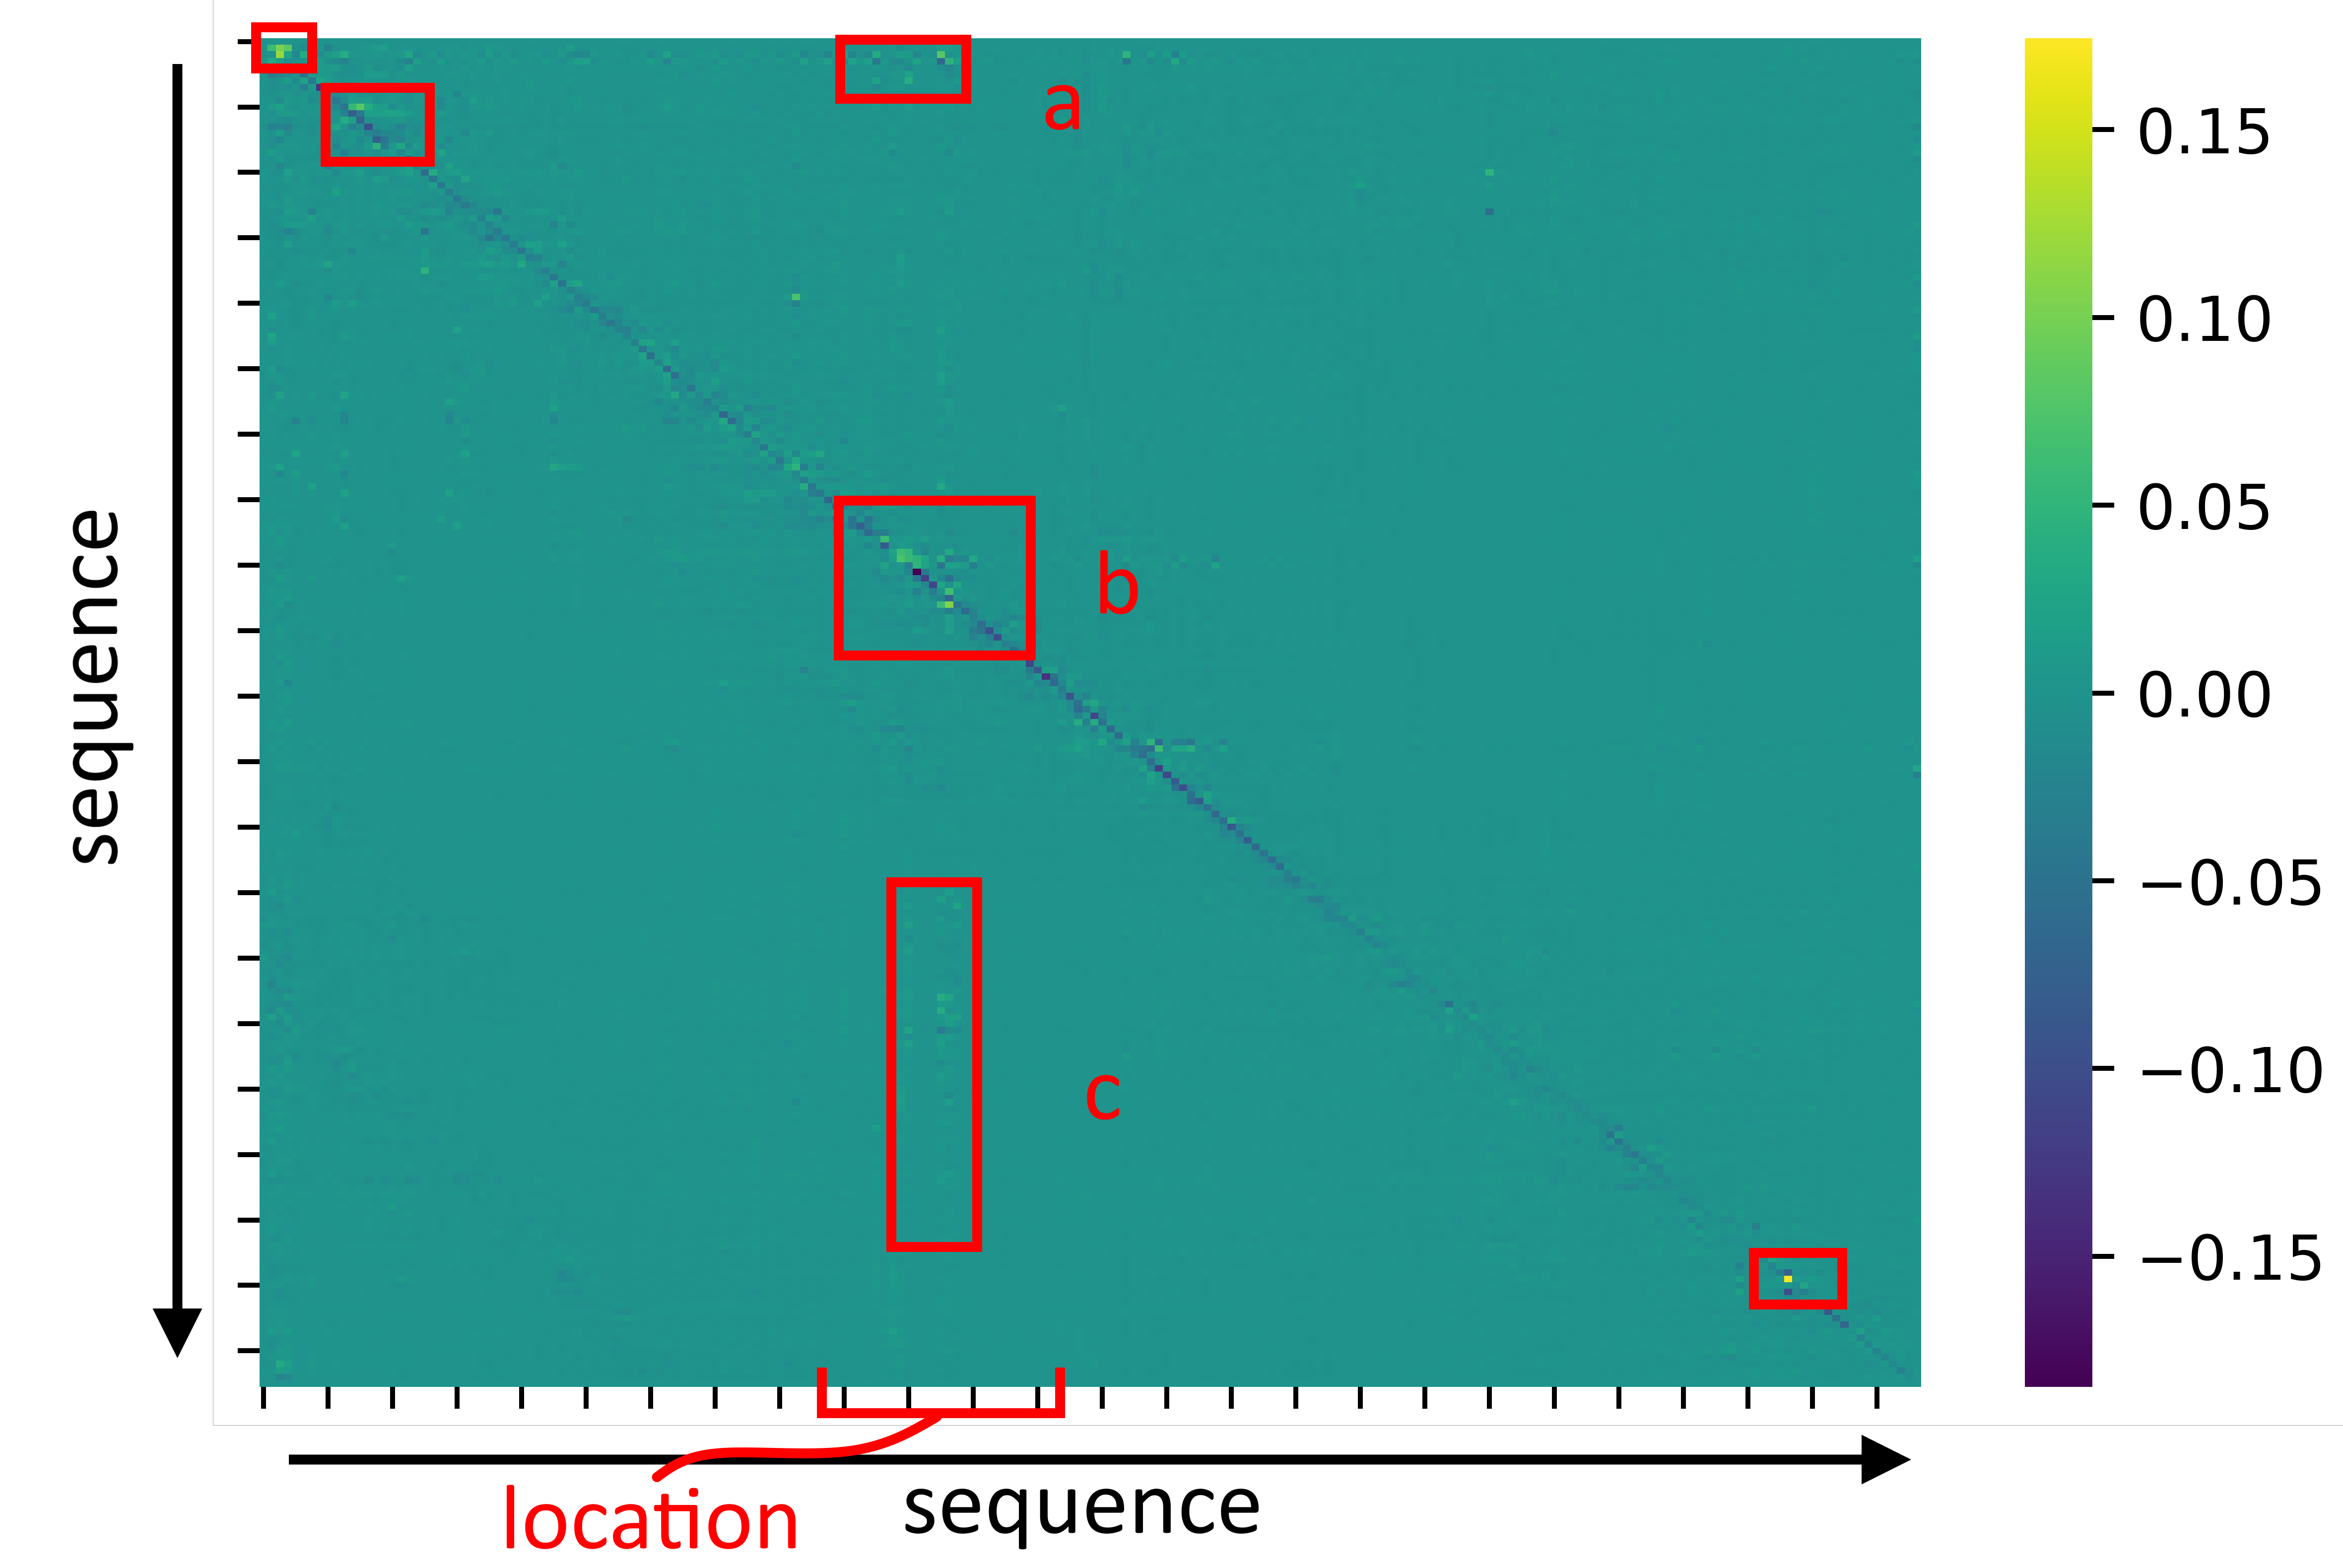
\includegraphics[width=0.75\textwidth]{sequence_shap_map_loc_annot.png}
\label{shap_mt_alloc}
\end{figure}
\newline
Далее возможно восстановить оригинальные слова из токенов с наивысшими значениями и полноценно описать их контекстуальное значение при выделении региона с диагнозом.
\newline
Таким образом, построение таких матриц позволяет пронаблюдать работу с контекстом внутри алгоритма, вывести логику принятия решения и оценить ее правомерность экспертом.
\section{Заключение}
В ходе работы были собраны основные статьи и технологии, отметившиеся в сфере решения задач обработки ествественного языка. Подробно описана проблематика и специфика задач этой области. Сформулированы основные свойства вложенных многомерных представлений данных в текстовой модальности, разобраны токенизация и векторизация текста.
\newline
Был сделал обзор истории развития архитектур, применяемых в области NLP. Изучена парадигма проектирования сетей "энкодер-декодер", общая методология работы с данными неопределенной размерности и механизм внимания, а также архитектура "трансформер" на его основе. Разобрана технология претренеровки двунаправленных трансформеров для понимая текста.
\newline
Используя фреймворки pytorch, numpy и hugging face transformers была решена задача бинарной классификации токенов на медецинском датасете NBME. Обучение позволило получить модель с показателем метрики в ~10\% окрестности текущего SOTA решения, пригодную для дальнейшей интерпретации.
\newline
При помощи выбранной методики SHAP были проанализированы взаимосвязи между токенами одной последовательности при обработке натренерованной моделью. Был предложен метод визуализации на основе матриц значений SHAP, показывающий контекстуальную роль токенов. Также метод предпологает возможность дальнейшего соотнесения полученных зависимостей с оригинальными токенами и словами, то есть возможность восстановить логику принятия решения алгоритмом.

% библиография
\newpage
\begin{thebibliography}{}
    \bibitem{w2v} Tomas Mikolov, Kai Chen, Greg Corrado, Jeffrey Dean. “Efficient Estimation of Word Representations in Vector Space.” (2013).
    \bibitem{ft} Piotr Bojanowski, Edouard Grave, Armand Joulin, Tomas Mikolov. “Enriching Word Vectors with Subword Information.” (2017).
    \bibitem{transformer} Ashish Vaswani, Noam Shazeer, Niki Parmar, Jakob Uszkoreit, Llion Jones, Aidan N. Gomez, Lukasz Kaiser, Illia Polosukhin. “Attention Is All You Need.” (2017).
    \bibitem{bert} Jacob Devlin, Ming-Wei Chang, Kenton Lee, Kristina Toutanova. “BERT: Pre-training of Deep Bidirectional Transformers for Language Understanding.” (2018).
    \bibitem{bpe} Philip Gage. “A New Algorithm for Data Compression.” (1994).
    \bibitem{med_survey} Geert Litjens, Thijs Kooi, Babak Ehteshami Bejnordi, Arnaud Arindra Adiyoso Setio, Francesco Ciompi, Mohsen Ghafoorian, Jeroen A.W.M. van der Laak, Bram van Ginneken, Clara I. Sanchez. “A Survey on Deep Learning in Medical Image Analysis.” (2017).
    \bibitem{word_piece} Mike Schuster, Kaisuke Nakajima, "Japanese and Korean voice search." (2012)
    \bibitem{pe} Kazemnejad Amirhossein, "Transformer Architecture: The Positional Encoding." (2019)
    \bibitem{RNN_survey} Zachary C. Lipton, John Berkowitz, Charles Elkan "A Critical Review of Recurrent Neural Networks for Sequence Learning." (2015)
    \bibitem{LSTM} Sepp Hochreiter, J¨urgen Schmidhuber "Long short-term memory." (1997)
    \bibitem{Attention} Dzmitry Bahdanau, Kyung Hyun Cho, Yoshua Bengio "Neural Machine Translation by Jointly Learning to Align and Translate." (2014)
    \bibitem{NBME} https://www.kaggle.com/competitions/nbme-score-clinical-patient-notes (2022)
    \bibitem{model_expl} Scott M. Lundberg, Su-In Lee "A Unified Approach to Interpreting Model Predictions." (2017)
    \bibitem{shap_models} Mukund Sundararajan, Amir Najmi "The Many Shapley Values for Model Explanation." (2020)
    \bibitem{bert_shap} Blaz Skrlj, Shane Sheehan, Nika Erzen, Marko Robnik-Sikonja, Saturnino Luz, Senja Pollak "BERT meets Shapley: Extending SHAP Explanations to Transformer-based Classifiers." (2020)
\end{thebibliography}
% добавляем библиографию в содержание
\addcontentsline{toc}{section}{Список используемой литературы}

%приложения
\newpage
\include{addition}
\end{document}